\documentclass[10pt]{beamer}
\usepackage{graphicx}
\usepackage[german]{babel}
\usepackage{qtree}
\usepackage{xcolor}
\usepackage[style=numeric-verb]{biblatex}
\bibliographystyle{plain}
%\bibliography{Quellen}
\addbibresource{Quellen.bib}


\usetheme[left]{AAUsidebar}



\usepackage[utf8]{inputenc}
\usepackage[T1]{fontenc}
% Or whatever. Note that the encoding and the font should match. If T1
% does not look nice, try deleting the line with the fontenc.
\usepackage{helvet}

% colored hyperlinks
\newcommand{\chref}[2]{%
  \href{#1}{{\usebeamercolor[bg]{AAUsidebar}#2}}%
}

\title[Semantic Argument Classification]% optional, use only with long paper titles
{Semantic Argument Classification}

%\subtitle{v.\ 1.3.0}  % could also be a conference name

\date{28. Januar 2015}

\author[Julian Baumann, Kevin Decker, Maximilian Müller-Eberstein] % optional, use only with lots of authors
{
    Julian Baumann, Kevin Decker, Maximilian Müller-Eberstein
  %email adress
  %\href{mailto:jkn@es.aau.dk}{{\tt jkn@es.aau.dk}}
}
% - Give the names in the same order as they appear in the paper.
% - Use the \inst{?} command only if the authors have different
%   affiliation. See the beamer manual for an example

\institute[
%  {\includegraphics[scale=0.2]{aau_segl}}\\ %insert a company, department or university logo
  Institut für Computerlinguistik\\
  Ruprecht-Karls-Universität Heidelberg\\
  
] % optional - is placed in the bottom of the sidebar on every slide
{% is placed on the title page
  Institut für Computerlinguistik\\
  Universität Heidelberg\\

  %there must be an empty line above this line - otherwise some unwanted space is added between the university and the country (I do not know why;( )
}


% specify a logo on the titlepage (you can specify additional logos an include them in 
% institute command below
%\pgfdeclareimage[height=1.5cm]{titlepagelogo}{uniHeidelberg} % placed on the title page
%\pgfdeclareimage[height=1.5cm]{titlepagelogo2}{graphics/aau_logo_new} % placed on the title page
\titlegraphic{% is placed on the bottom of the title page
  
\includegraphics[height=1.5cm]{AAUgraphics/uniHeidelberg}
%  \hspace{1cm}\pgfuseimage{titlepagelogo2}
}


\begin{document}

%\lstset{language=Python}
% the titlepage
{\aauwavesbg%
\begin{frame}[plain,noframenumbering] % the plain option removes the sidebar and header from the title page
  \titlepage
\end{frame}}
%%%%%%%%%%%%%%%%%%%%%%%%%%%%%%%%%%%%

% TOC
\begin{frame}{Gliederung}{}
\small{\tableofcontents}
\end{frame}
%%%%%%%%%%%%%%%%%%%%%%%%%%%%%%%%%%%%%

\section{Problemstellung}

\begin{frame}{Semantic Argument Classification}{}
  \textbf{Was ist Semantic Argument Classifcation?}
  \vspace{5pt}
  
  \begin{itemize}
    \item Zuweisung bestimmter Rollen in einem Satz $\Rightarrow$ \\
    \glqq{}Wer tut wem was an?\grqq{}
    \item It operates stores mostly in Iowa and Nebraska
    \item $ [_{\textbf{Arg0}} It][_{\textbf{Pred}} operates][_{\textbf{Arg1}} stores] [_{\textbf{ArgLoc}} mostly\ in\ Iowa\\ \hspace{20pt} and\ Nebraska]$
  \end{itemize}
\end{frame}

\subsection{Anwendungsbereich}
%%%%%%%%%%%%%%%%%%%%%%%%%%%%%%%%%%%%%%
\section{Daten}
\begin{frame}{Daten}
  \begin{itemize}
   \item NLTK
   \item PropBank
  \end{itemize}

\end{frame}

\begin{frame}{PropBank}
  \begin{itemize}
   \item versucht generalisierte Argumente zu verwenden $\rightarrow$ Parser
   \item Argumentrollen sind für jedes Verb in Frames organisiert $\rightarrow$ weniger spezifisch
   \item ARG0 = Proto-Agent
   \item ARG1 = Proto-Patient
   \item ARG2-ARG5 = Argumente mit steigender Intensität
   % He(Arg0) wrote(Predicate) a book(Arg1) 
   % He wrote about them(Arg2) (intensiver, anderer Sense)
   % He wrote a book for his children (Arg3) weiter entfernt 
   % verschiedene Rollen
  \end{itemize}
\end{frame}


\begin{frame}{Penn Treebank}
  \begin{itemize}
   \item Subkorpus aus WSJ und Brown Corpus, bestehend aus ungefähr 1.000.000 Wörtern
   \item 112.917 Prädikat-Argument Strukturen annotiert nach PropBank-Annotationsschema
   \item 292.975 Instanzen
   \item wsj/00/wsj\_0001.mrg 1 10 gold publish.01 p---a 10:0-rel 11:0-ARG0
          
  \end{itemize}
  
\end{frame}

\begin{frame}{Penn Treebank}
((S \\
\hspace{10pt}   (NP-MNR-SBJ \\
\hspace{25pt}   (NP (DT The) (NN way) ) \\
\hspace{25pt} (SBAR \\
\hspace{40pt}  (WHADVP-1 (-NONE- 0) )\\
\hspace{40pt}   (S \\
\hspace{60pt}      (NP-SBJ (NNP MacArthur) )\\
\hspace{60pt}    (VP (VBD said) \\
\hspace{80pt}       (NP (PRP his) (NN line) )\\
\hspace{80pt}      (ADVP-MNR (-NONE- *T*-1) )))))\\
 (: - -) \\
    

\end{frame}

\subsection{Problemstellung}
%%%%%%%%%%%%%%%%%%%%%%%%%%%%%%%%%%%%%%%

%Todo: Bilder für Klassenverteilung und Features einfügen: PhraseType, Postion, Voice
\section{Umsetzung}
\subsection{Features}
  \begin{frame}{Features}
    \begin{itemize}
     \item Predicate
     \item Path
     \item Phrase Type
     \item Position
     \item Voice
    \end{itemize}
    \begin{figure}
     	\begin{center}
    		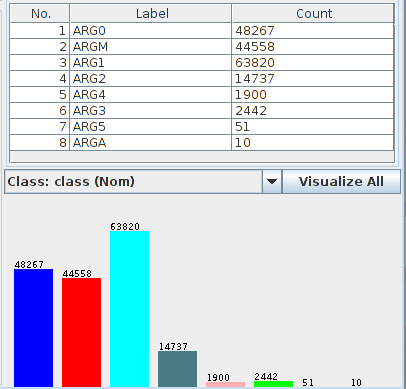
\includegraphics[scale=0.3]{class}
    	\end{center}
    
    \end{figure}
    
   \end{frame}
   
  \begin{frame}{Predicate}
    \begin{itemize}
     \item lemmatisierte Prädikat
     \item 3966 distinct
    \end{itemize} 
  \end{frame}
  
  \begin{frame}{Path}
  \begin{itemize}
   \item beschreibt Pfad zwischen ARG und Predicate 
   \item vereinfacht z.B. NP-SBJ $\rightarrow$ NP 
   \item extrahiert über Lowest Common Ancestor 
   \item beispielsweise: NP$\uparrow$S$\downarrow$VP$\downarrow$VBD
   \item 41737 distinct
  \end{itemize}

   \Tree [.S [\qroof{The lawyers\\ \textbf{ARG0}}.NP  ] [.VP [.VBD {went\\ \textbf{Predicate}} ] [.PP {to\\ \textbf{Null}} ] [.NP {work\\ \textbf{ARG4}} ] ] ]
  \end{frame}

  \begin{frame}{Phrase Type}
   \begin{itemize}
    \item beschreibt die Kategorie des Argument
    \item z.B: NP, MD, PP, SBAR
    \item 65 distinct feature values
   \end{itemize}
   
   \begin{figure}
   	\begin{center}
   		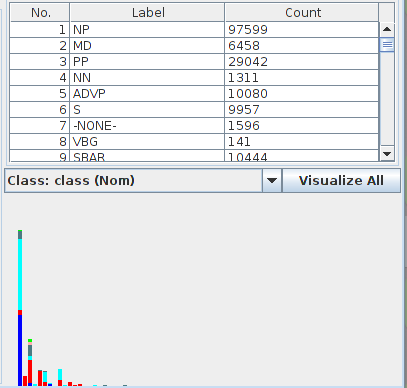
\includegraphics[scale=0.3]{phraseType}
   	\end{center}
   \end{figure}
  \end{frame}
  
  \begin{frame}{Position}
   \begin{itemize}
    \item Beschreibt, ob das Argument vor oder nach dem Prädikat steht
    \item ninäres Feature
   \end{itemize}
   
   \begin{figure}
   	\begin{center}
   		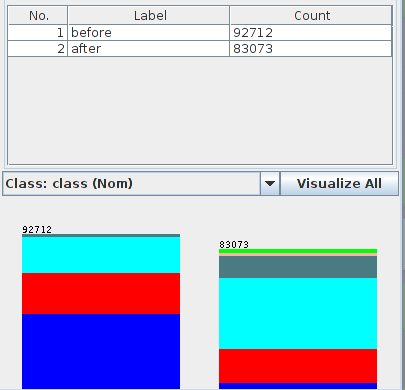
\includegraphics[scale=0.3]{position}
   	\end{center}
   \end{figure}
  \end{frame}
  
  \begin{frame}{Voice}
   \begin{itemize}
    \item gibt an, ob das Prädikat aktiv oder passiv ist
    \item größtenteils annotiert
    \item 3 distinct feature values: active, passive, unknown
   \end{itemize}
  \begin{figure}
	  \begin{center}
	  	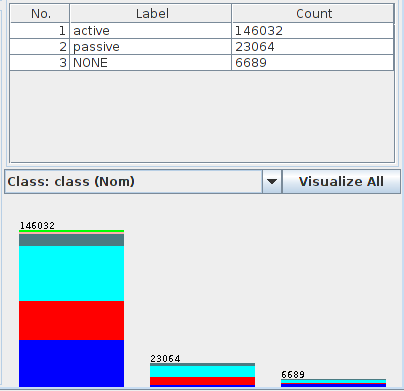
\includegraphics[scale=0.3]{voice}
	  \end{center}
  \end{figure}
  \end{frame}
  



\subsection{Featureextraktion}

\begin{frame}{Featureextraktion} 
\begin{small}
\hspace{10pt} featureList = $[$...$]$ \textcolor{lightgray}{\# zu extrahierende Features} \\
\hspace{10pt} extArgList = [] \\
\hspace{10pt} for pbInstance in pbInstances : \\
\hspace{30pt} 	for pbArg in pbInstance.arguments : \\
\hspace{30pt} 	for feature in featureList : \\
\hspace{50pt}	extArgList.append(extFeature(feature, pbArg, pbInstance)) \\
\hspace{10pt}   	\textcolor{lightgray}{ \# write features to file in ARFF} \\
\end{small}
\end{frame}

\begin{frame}{Featureextraktion} 
  \begin{figure}
	  \begin{center}
	  	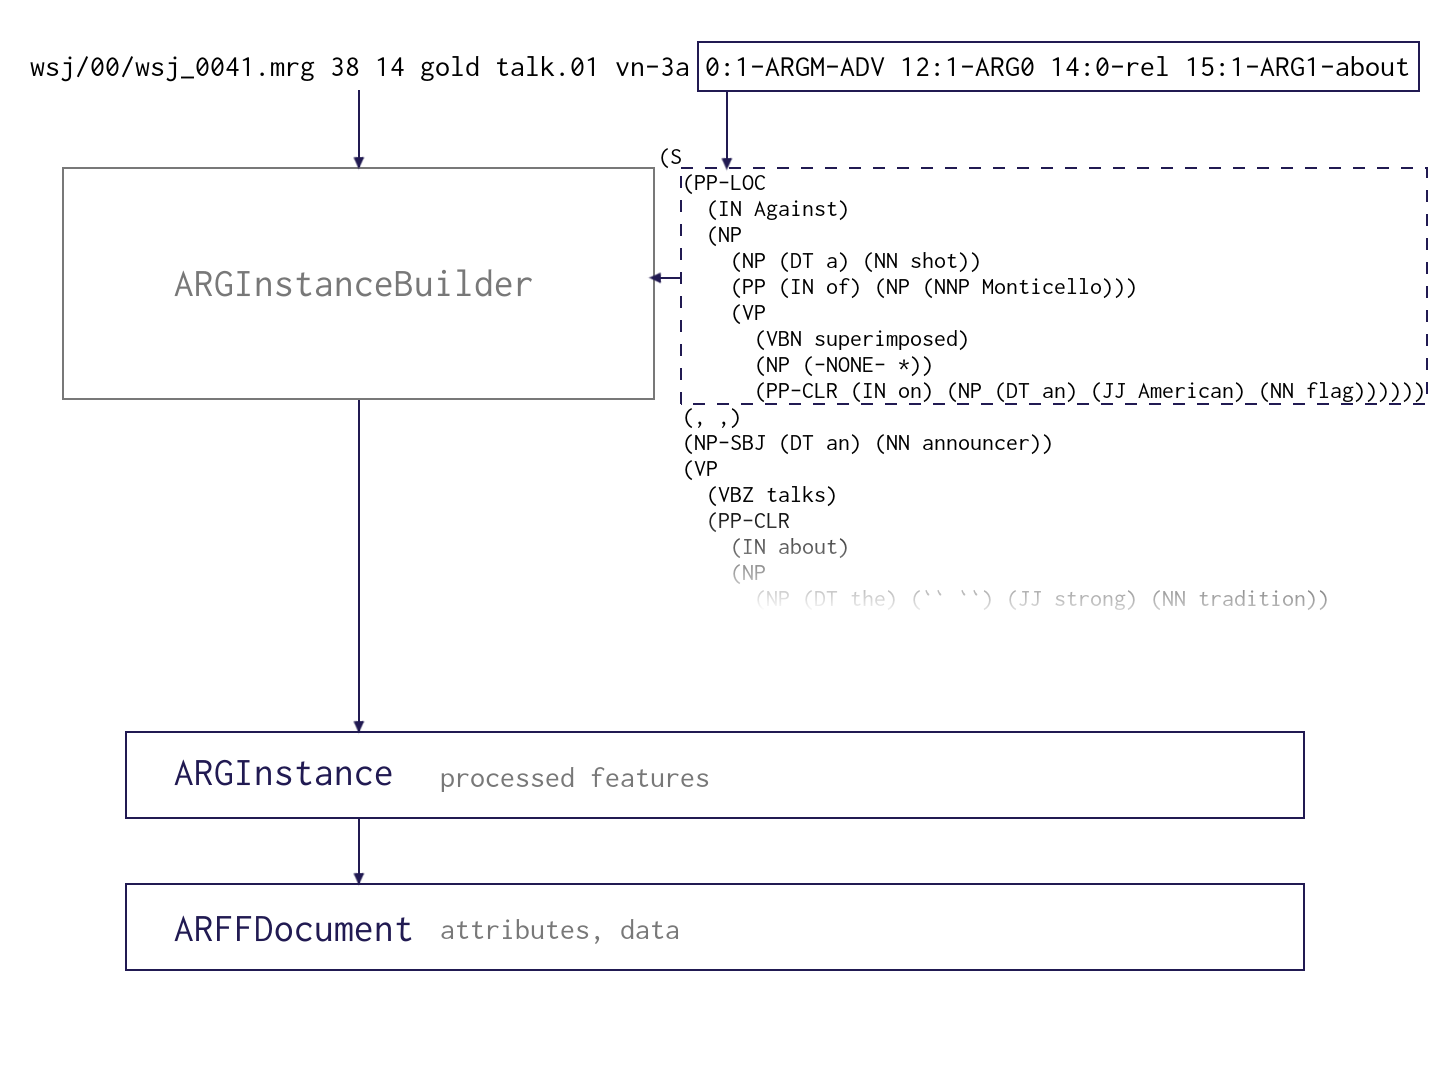
\includegraphics[scale=0.5]{argext_graphic}
	  \end{center}
  \end{figure}
\end{frame}

\begin{frame}{ARFF}
	@relation SAC\_All \\
	\vspace{5pt}
	@attribute predicate \{join,publish,name,use, make, cause, ...\} \\
	@attribute phraseType \{NP, MD, PP, NN, ADVP, S, ...\} \\
	@attribute position \{before, after\} \\
	@attribute path \{NP\^{}S!VP!VP, MD\^{}VP\^{}S!VP!VP,...\} \\
	@attribute voice \{active, passive, NONE\} \\
	@attribute class \{ARG0, ARGM, ARGA, ARG1, ...\} \\
	\vspace{10pt}
	@data \\
	join, NP, before, NP\^{}S!VP!VP, active, ARG0 \\
	join, MD, before, MD\^{}VP\^{}S!VP!VP, active, ARGM \\
	join, NP, after, NP\^{}VP\^{}VP\^{}S!VP!VP, active, ARG1 \\
	join, PP, after, PP\^{}VP\^{}VP\^{}S!VP!VP, active, ARGM \\
	join, NP, after, VP\^{}VP\^{}S!VP!VP, active, ARGM \\

\end{frame}



%%%%%%%%%%%%%%%%%%%%%%%%%%%%%%%%%%%%%%
\subsection{Schwierigkeiten}
%%%%%%%%%%%%%%%%%%%%%%%%%%%%%%%%%%%%%%
\section{Experimente}
\begin{frame}{Setup}

\begin{itemize}
	\item 60\% train,20\% dev, 20\% test
	\item Baseline: ZeroR
	\item Naive Bayes, j48 tree, \textit{(libSVM)} 
	\item bisher: Training auf train, Evaluierung mit dev
\end{itemize}

\end{frame}

\begin{frame}{Ergebnisse}
\begin{table}[h]
\begin{tabular}{l|lll}
                  & Precision      & Recall         & F-Measure      \\ \hline
\textit{Baseline} & \textit{0.132} & \textit{0.364} & \textit{0.194} \\ \hline
Naive Bayes       & 0.771          & 0.778          & 0.770          \\
j48 Tree          & 0.784      	   & 0.786             & 0.781            
\end{tabular}
\end{table}
\end{frame}

\begin{frame}{Feature Evaluation}

\begin{frame}{Confusion Matrix (Naive Bayes)}

\begin{table}[h]
\begin{tabular}{llllllll|l}
a     & b     & c     & d    & e   & f  & g & h & \textless-- classified as \\ \hline
14497 & 348   & 361   & 272  & 0   & 4  & 0 & 1 & a = ARG0                  \\
291   & 11394 & 2143  & 1009 & 189 & 48 & 0 & 1 & b = ARGM                  \\
3119  & 707   & 17064 & 375  & 31  & 27 & 0 & 0 & c = ARG1                  \\
180   & 792   & 1854  & 2163 & 29  & 23 & 0 & 0 & d = ARG2                  \\
2     & 217   & 23    & 141  & 379 & 3  & 0 & 0 & e = ARG3                  \\
37    & 289   & 144   & 147  & 170 & 99 & 0 & 0 & f = ARG4                  \\
0     & 13    & 0     & 1    & 0   & 0  & 3 & 0 & g = ARG5                  \\
5     & 0     & 0     & 0    & 0   & 0  & 0 & 0 & h = ARGA                 
\end{tabular}
\end{table}
\end{frame}

\begin{table}[h]
\begin{tabular}{l|lll|l}
                      & Precision      & Recall         & F-Measure      & F-Measure Change \\ \hline
\textit{All Features} & \textit{0.771} & \textit{0.778} & \textit{0.770} & \textit{0}       \\ \hline
- voice               & 0.748          & 0.754          & 0.745          & -0.025           \\
- path                & 0.778          & 0.783          & 0.776          & \textbf{+0.006}  \\
- phraseType          & 0.735          & 0.747          & 0.733          & -0.037           \\
- position            & 0.758          & 0.773          & 0.757          & -0.013           \\
-predicate            & 0.717          & 0.732          & 0.716          & \textbf{-0.54}  
\end{tabular}
\end{table}

\end{frame}



%%%%%%%%%%%%%%%%%%%%%%%%%%%%%%%%%%%%%%
\section{Ausblick}

\begin{frame}{toDo}

\begin{itemize}
	\item Path Feature überarbeiten
	\item HeadWord Feature implementieren
	\item genauere Evaluation
	\item \textit{SVM?}
	\item Abschlussbericht schreiben

\end{itemize}
%%%%%%%%%%%%%%%%%%%%%%%%%%%%%%%%%%%%%
\section{Literatur}
\begin{frame}{Quellen}
    \renewcommand*{\refname}{Referenzen}
    \nocite{*} 
    \printbibliography 
\end{frame} 

{\aauwavesbg
\begin{frame}[plain,noframenumbering]
  \finalpage{Vielen Dank für Eure Aufmerksamkeit! \\ Noch Fragen?}
\end{frame}
%%%%%%%%%%%%%%%%

\end{document}
